\newpage
\section{IMPLEMENTATION}

With the proposed objective and methodology, the pathway was implemented almost similar to what was proposed.

\begin{itemize}
	\item Within the first week of undertaking the project, project was chosen and thus,
	subsequently a rough path was discussed and project proposal was made.
	\item After the project proposal, a rough sketch of the project schedule was
	created.
	\item Since three of our contributor were on three different OS(Windows, MacOS and Linux) we had to spend about a week or two to configure CMake for making our game cross-platform.
	\item Then we thoroughly studied and used the SFML Starter-Kit TheStateMachine for managing different pages in the game in most efficient way possible.
	\item Then we focused on the Core Game-Logic
	\item Then we added Multimedia resources like Tetromino, Grid, photos for different buttons.
	\item We added FileManager Class which updated the Score and retrieved the score from a file.
	\item Sound was Added to the Game.
	\item Final Code was tested and debugged
	\item Final Program was documented and a presentation was prepared.
\end{itemize}

\begin{figure}[H]
	\centering
	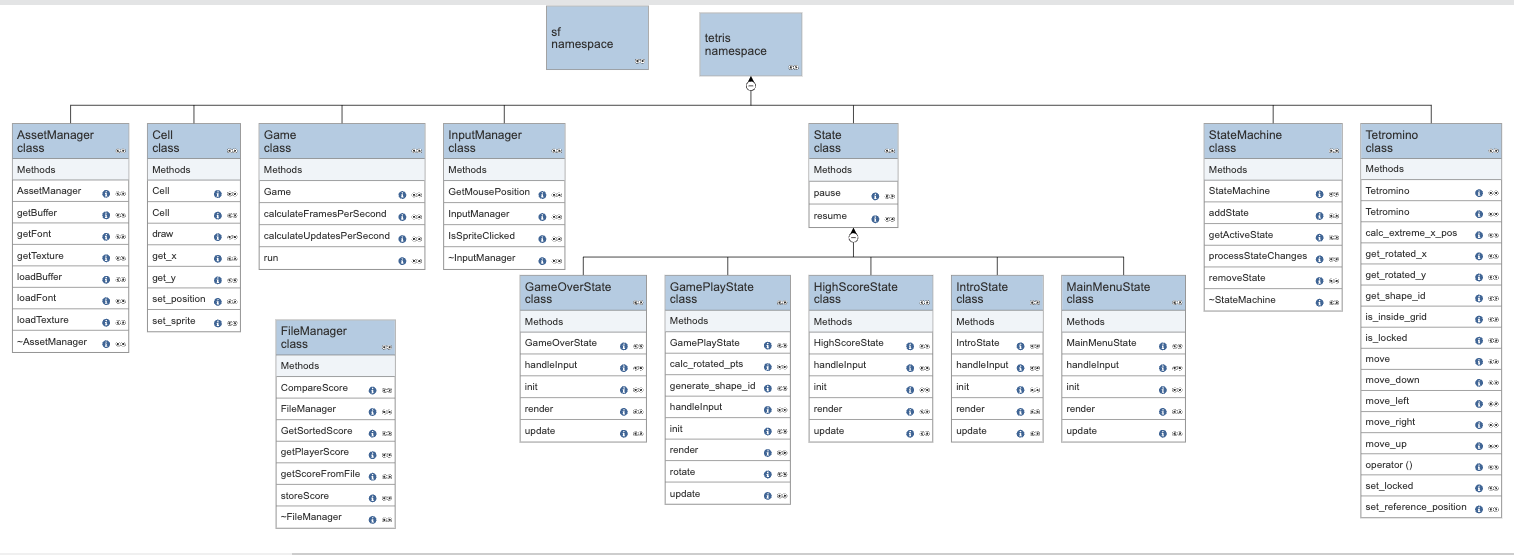
\includegraphics[width=1.2\textwidth]{images/ClassDiagram}
	\caption{Class Diagram of the Game}
\end{figure}


\begin{figure}[H]
	\centering
	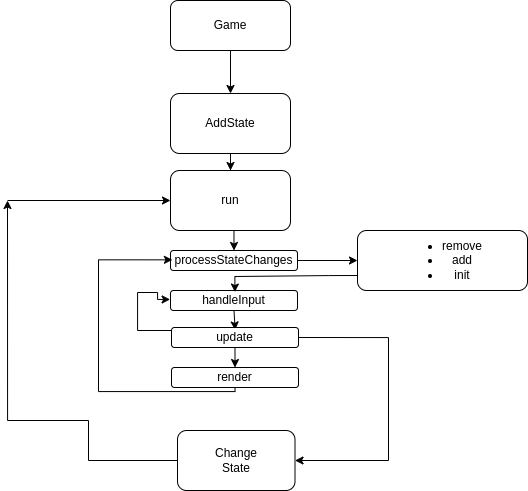
\includegraphics[width=0.7\textwidth]{images/StateMachine.png}
	\caption{Block Diagram: State Machine}
\end{figure}

\begin{figure}[H]
	\centering
	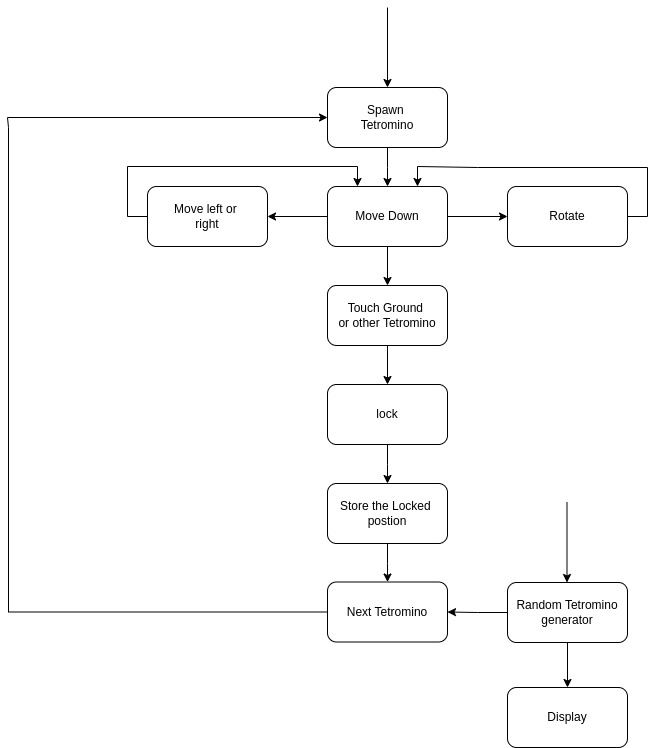
\includegraphics[width=0.7\textwidth]{images/GamePlayBlockDiagram.jpg}
	\caption{Block Diagram: GamePlay}
\end{figure}

